\documentclass[11pt]{beamer}
\usetheme{Antibes}
\usepackage{ragged2e}
\usepackage {tikz}
\usetikzlibrary{positioning}
\definecolor {processblue}{cmyk}{0.96,0,0,0}
\title{FTech Training}
\subtitle{Using Beamer}
\author{Luc Nguyen}
\institute{HUST}
\date{\today}
\usetheme{Boadilla}
\begin{document} % auto-compile by Ctrl + S
	\begin{frame}
		\frametitle{\textbf{CONVOLUTIONAL NEURAL NETWORK}}
		\framesubtitle{}
		\begin{itemize}
			\item mka 
			\item alksmd
		\end{itemize}
		\begin{center}
		\begin{math}
				\dfrac{\pi\log_3x^2+2}{\sum\sqrt[3]{x^4}+e^5}
			\end{math}
		\end{center}
	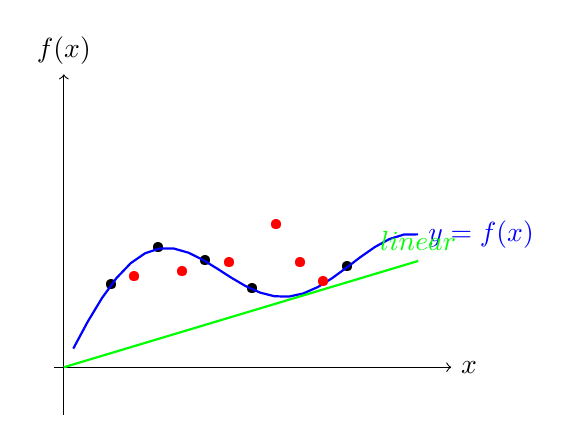
\begin{tikzpicture}[domain=0:8, scale=0.6]
\draw[->] (-0.2,2) -- (8.2,2) node[right] {$x$};
\draw[->] (0,1.0) -- (0,8.2) node[above] {$f(x)$};
\foreach \Point in {(1, 3.741), (2, 4.509), (3, 4.2411), (4, 3.643), (6, 4.120) }{
    \node at \Point {\textbullet};
}
\pause
\draw[color=blue, thick, domain=0.2:7.5] plot(\x,{-\x^2/10+\x+2+sin(\x r)}) node[right] {$y = f(x)$} ;
\draw[color=green, thick, domain=0:7.5] plot(\x, {\x*0.3 + 2}) node[right, above] {$linear$};

\foreach \Point in {(1.5, 3.9), (2.5, 4), (3.5, 4.2), (4.5, 5), (5, 4.2), (5.5, 3.8) }{
    \node at \Point {\color{red}\textbullet};
}
	\end{tikzpicture}	
\end{frame}

\end{document}